\documentclass[12pt]{article}
\input{/Users/circle/Documents/博一下/homework/setting.tex}
\setcounter{secnumdepth}{2}
\usepackage{autobreak}
\usepackage{amsmath}
\setlength{\parindent}{2em}
\graphicspath{{../}}
\ziju{0.1pt}

%pdf文件设置
\hypersetup{
	pdfauthor={袁磊祺},
	pdftitle={计算流体力学作业6}
}

\title{
		\vspace{-1in} 	
		\usefont{OT1}{bch}{b}{n}
		\normalfont \normalsize \textsc{\LARGE Peking University}\\[0.2cm] % Name of your university/college \\ [25pt]
		\horrule{0.5pt} \\[0.2cm]
		\huge \bfseries{计算流体力学作业6} \\[-0.2cm]
		\horrule{2pt} \\[0.2cm]
}
\author{
		\normalfont 								\normalsize
		College of Engineering \quad 2001111690  \quad 袁磊祺\\	\normalsize
        \today
}
\date{}

\begin{document}

%%%%%%%%%%%%%%%%%%%%%%%%%%%%%%%%%%%%%%%%%%%%%%
\captionsetup[figure]{name={图},labelsep=period}
\captionsetup[table]{name={表},labelsep=period}
\renewcommand\contentsname{目录}
\renewcommand\listfigurename{插图目录}
\renewcommand\listtablename{表格目录}
\renewcommand\refname{参考文献}
\renewcommand\indexname{索引}
\renewcommand\figurename{图}
\renewcommand\tablename{表}
\renewcommand\abstractname{摘\quad 要}
\renewcommand\partname{部分}
\renewcommand\appendixname{附录}
\def\equationautorefname{式}%
\def\footnoteautorefname{脚注}%
\def\itemautorefname{项}%
\def\figureautorefname{图}%
\def\tableautorefname{表}%
\def\partautorefname{篇}%
\def\appendixautorefname{附录}%
\def\chapterautorefname{章}%
\def\sectionautorefname{节}%
\def\subsectionautorefname{小小节}%
\def\subsubsectionautorefname{subsubsection}%
\def\paragraphautorefname{段落}%
\def\subparagraphautorefname{子段落}%
\def\FancyVerbLineautorefname{行}%
\def\theoremautorefname{定理}%
\crefname{figure}{图}{图}
\crefname{equation}{式}{式}
\crefname{table}{表}{表}
%%%%%%%%%%%%%%%%%%%%%%%%%%%%%%%%%%%%%%%%%%%

\maketitle

编写一维完全气体Euler方程组的LF格式, MacCormack 格式, 和一阶精度的显式迎风格式(Roe格式)的程序, 并计算讲义 (CFDLect04-com01_cn.pdf) 的第101-102页的问题2和问题4.

\begin{equation}
	\left\{\begin{array}{c}
	\left(\begin{array}{c}
	\rho \\
	\rho u \\
	E
	\end{array}\right)_{t}+\left(\begin{array}{c}
	\rho u \\
	\rho u^{2}+p \\
	u(E+p)
	\end{array}\right)_x=0, \\
	p=(\gamma-1)\left(E-\frac{1}{2} \rho u^{2}\right),\ \gamma=1.4.
	\end{array}\right.
\end{equation}

计算动图可点击 \href{https://www.bilibili.com/video/bv17N411f7tX}{https://www.bilibili.com/video/bv17N411f7tX} 查看。

代码可点击 \href{https://github.com/circlelq/Computational-Fluid-Dynamics/tree/main/code1}{https://github.com/circlelq/Computational-Fluid-Dynamics/tree/main/code1} 查看。


\section{1}

初始条件
\begin{equation}
	\boldsymbol{U}=\left\{\begin{array}{ll}
		(1,0,2.5)^{\mathrm{T}}, & x<0.3, \\
		(0.125,0,0.25)^{\mathrm{T}}, & x>0.3.
		\end{array}\right.
\end{equation}

计算区间为 $[0,1],$ 输出时刻 $t=0.2 .$

如\cref{fig:2ini} 所示为初始条件,密度$\rho$和压强$p$有一个初始间断,速度$u$都为0.之后的格式都采用固定CFL数,根据CFL数来求$\dif t$.其中$N$是$x$的网格数。之后的输出结果都是$t=0.2$时刻的结果,除非震荡剧烈,无法继续计算。

\begin{figure}[htp]
	\centering
	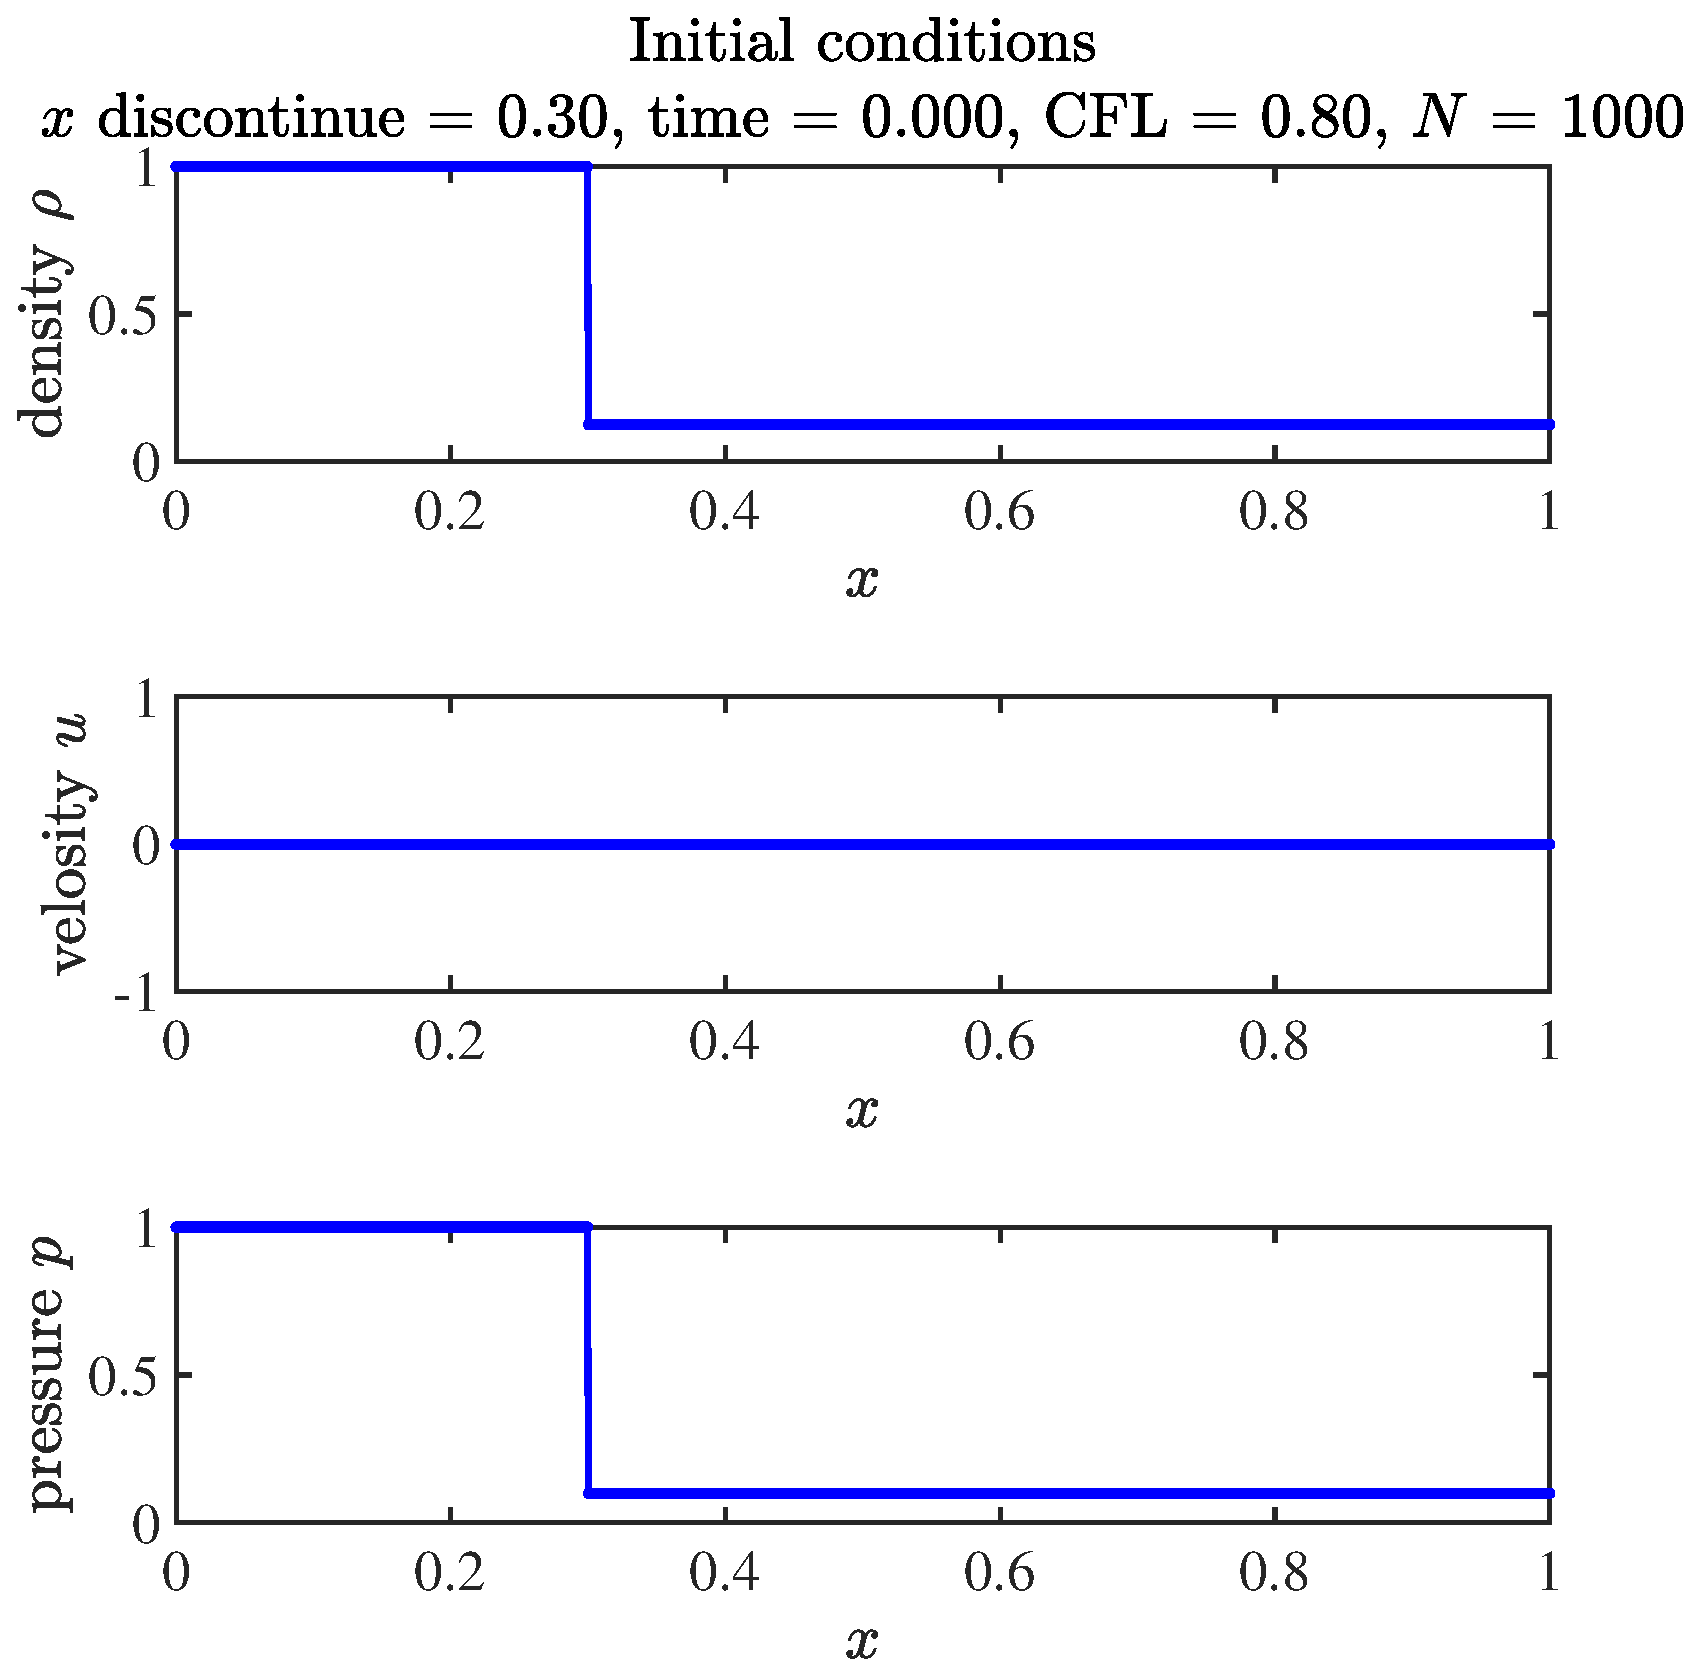
\includegraphics[width=9cm]{2Initial_conditions.eps}
	\vspace{20pt}
	\caption{初始条件。}
	\label{fig:2ini}
\end{figure}

\subsection{LF 格式}

\begin{equation}
	\bm{u}^{n+1}_{j} = \frac{1}{2} \left( \bm{u}^{n}_{j+1} + \bm{u}^{n}_{j-1} \right) - \frac{1}{2} r \left( \bm{f}^{n}_{j+1} - \bm{f}^{n}_{j-1} \right).
\end{equation}
其中$r=\tau/h$,稳定性条件为
\begin{equation}
	\abs{\bm{u}}_{\max} \frac{\tau}{h} \leqslant 1.
\end{equation}

如\cref{fig:2LF} 所示, LF格式是TVD的,所以无震荡。可以发现,计算结果为左边是一个稀疏波,中间是一个接触间断,右边是一个激波。
\begin{figure}[htp]
	\centering
	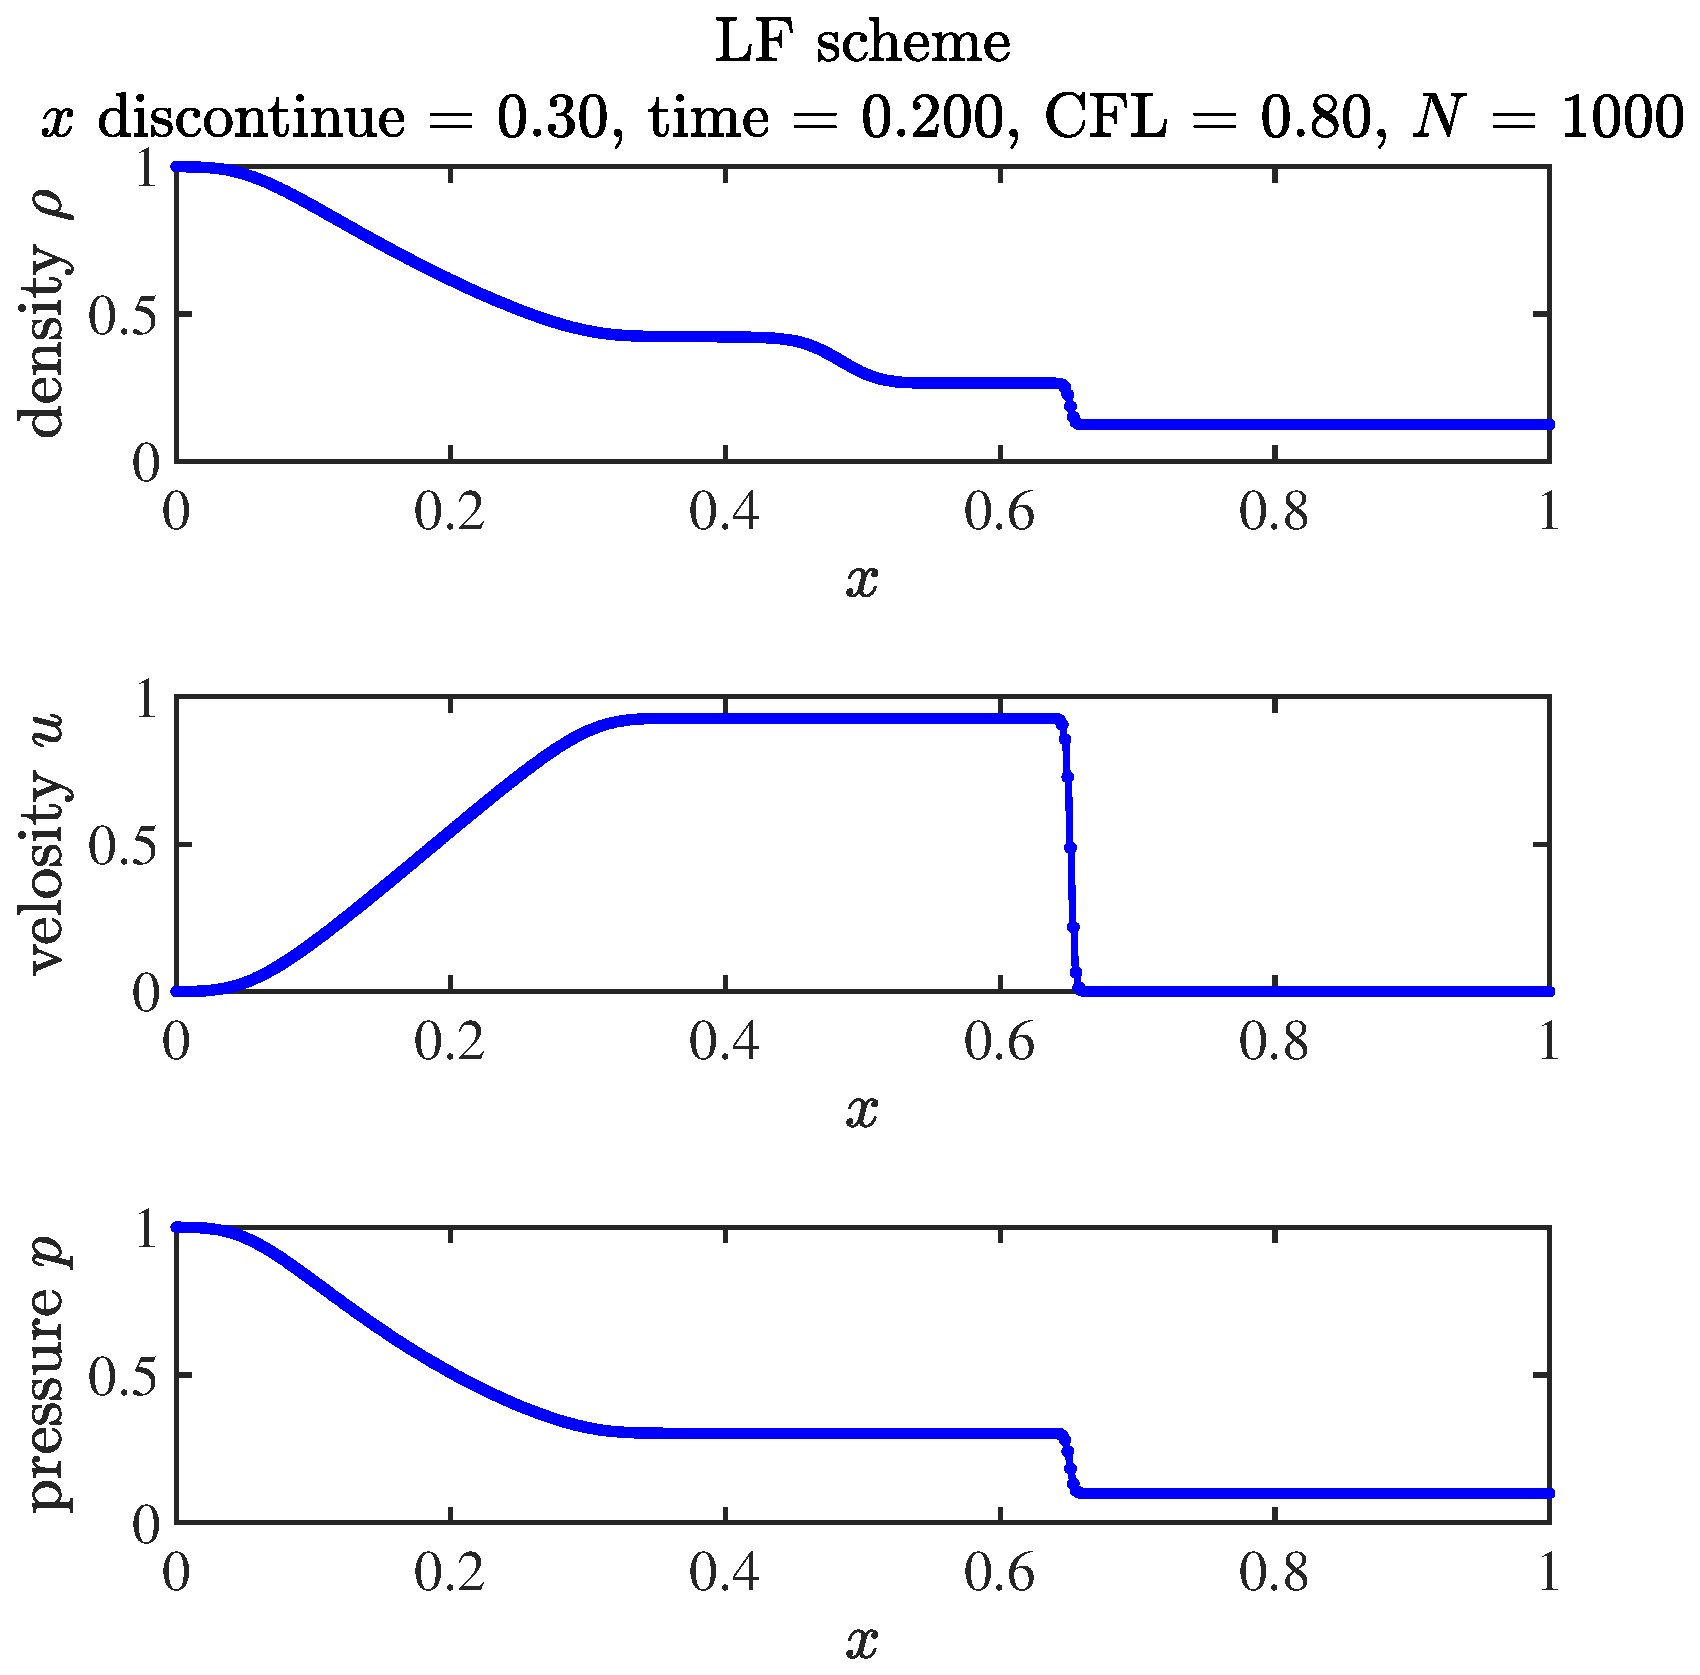
\includegraphics[width=9cm]{2LF.eps}
	\vspace{20pt}
	\caption{LF 格式计算结果。}
	\label{fig:2LF}
\end{figure}


\subsection{MacCormack格式}

MacCormack格式[R.W. MacCormack, AIAA Paper No. 1969-354 (1969)]
\begin{equation}
	\begin{aligned}
		u\left(x_{j}, t_{n+1}\right)=& u\left(x_{j}, t_{n}\right)+\tau\left(u_{t}\right)_{j}^{n}+\frac{1}{2} \tau^{2}\left(u_{t t}\right)_{j}^{n}+\mathcal{O}\left(\tau^{3}\right) \\
		=& \frac{1}{2} u\left(x_{j}, t_{n}\right)+\frac{1}{2}\left(\bar{u}+\tau \bar{u}_{t}\right)_{j}^{n}+\mathcal{O}\left(\tau^{3}\right), \quad \bar{u}:=u+\tau u_{t} 
		\end{aligned}
\end{equation}
\begin{equation}
		\left\{\begin{array}{l}
		\bar{u}_{j}^{*}=u_{j}^{n}-\frac{\tau}{h}\left(f\left(u_{j+1}^{n}\right)-f\left(u_{j}^{n}\right)\right), \\
		u_{j}^{n+1}=\frac{1}{2}\left(u_{j}^{n}+\bar{u}_{j}^{*}\right)-\frac{\tau}{2 h}\left(f\left(\bar{u}_{j}^{*}\right)-f\left(\bar{u}_{j-1}^{*}\right)\right).
		\end{array}\right.
\end{equation}
或
\begin{equation}
	\left\{\begin{array}{l}
		\bar{u}_{j}^{*}=u_{j}^{n}-\frac{\tau}{h}\left(f\left(u_{j}^{n}\right)-f\left(u_{j-1}^{n}\right)\right), \\
		u_{j}^{n+1}=\frac{1}{2}\left(u_{j}^{n}+\bar{u}_{j}^{*}\right)-\frac{\tau}{2 h}\left(f\left(\bar{u}_{j+1}^{*}\right)-f\left(\bar{u}_{j}^{*}\right)\right).
		\end{array}\right.
\end{equation}

如\cref{fig:2Mac} 所示, MacCormack格式震荡严重,导致$\dif t$只能取非常小的值,所以经过$300$步的计算后还是停留在$t=0.001$。

\begin{figure}[htp]
	\centering
	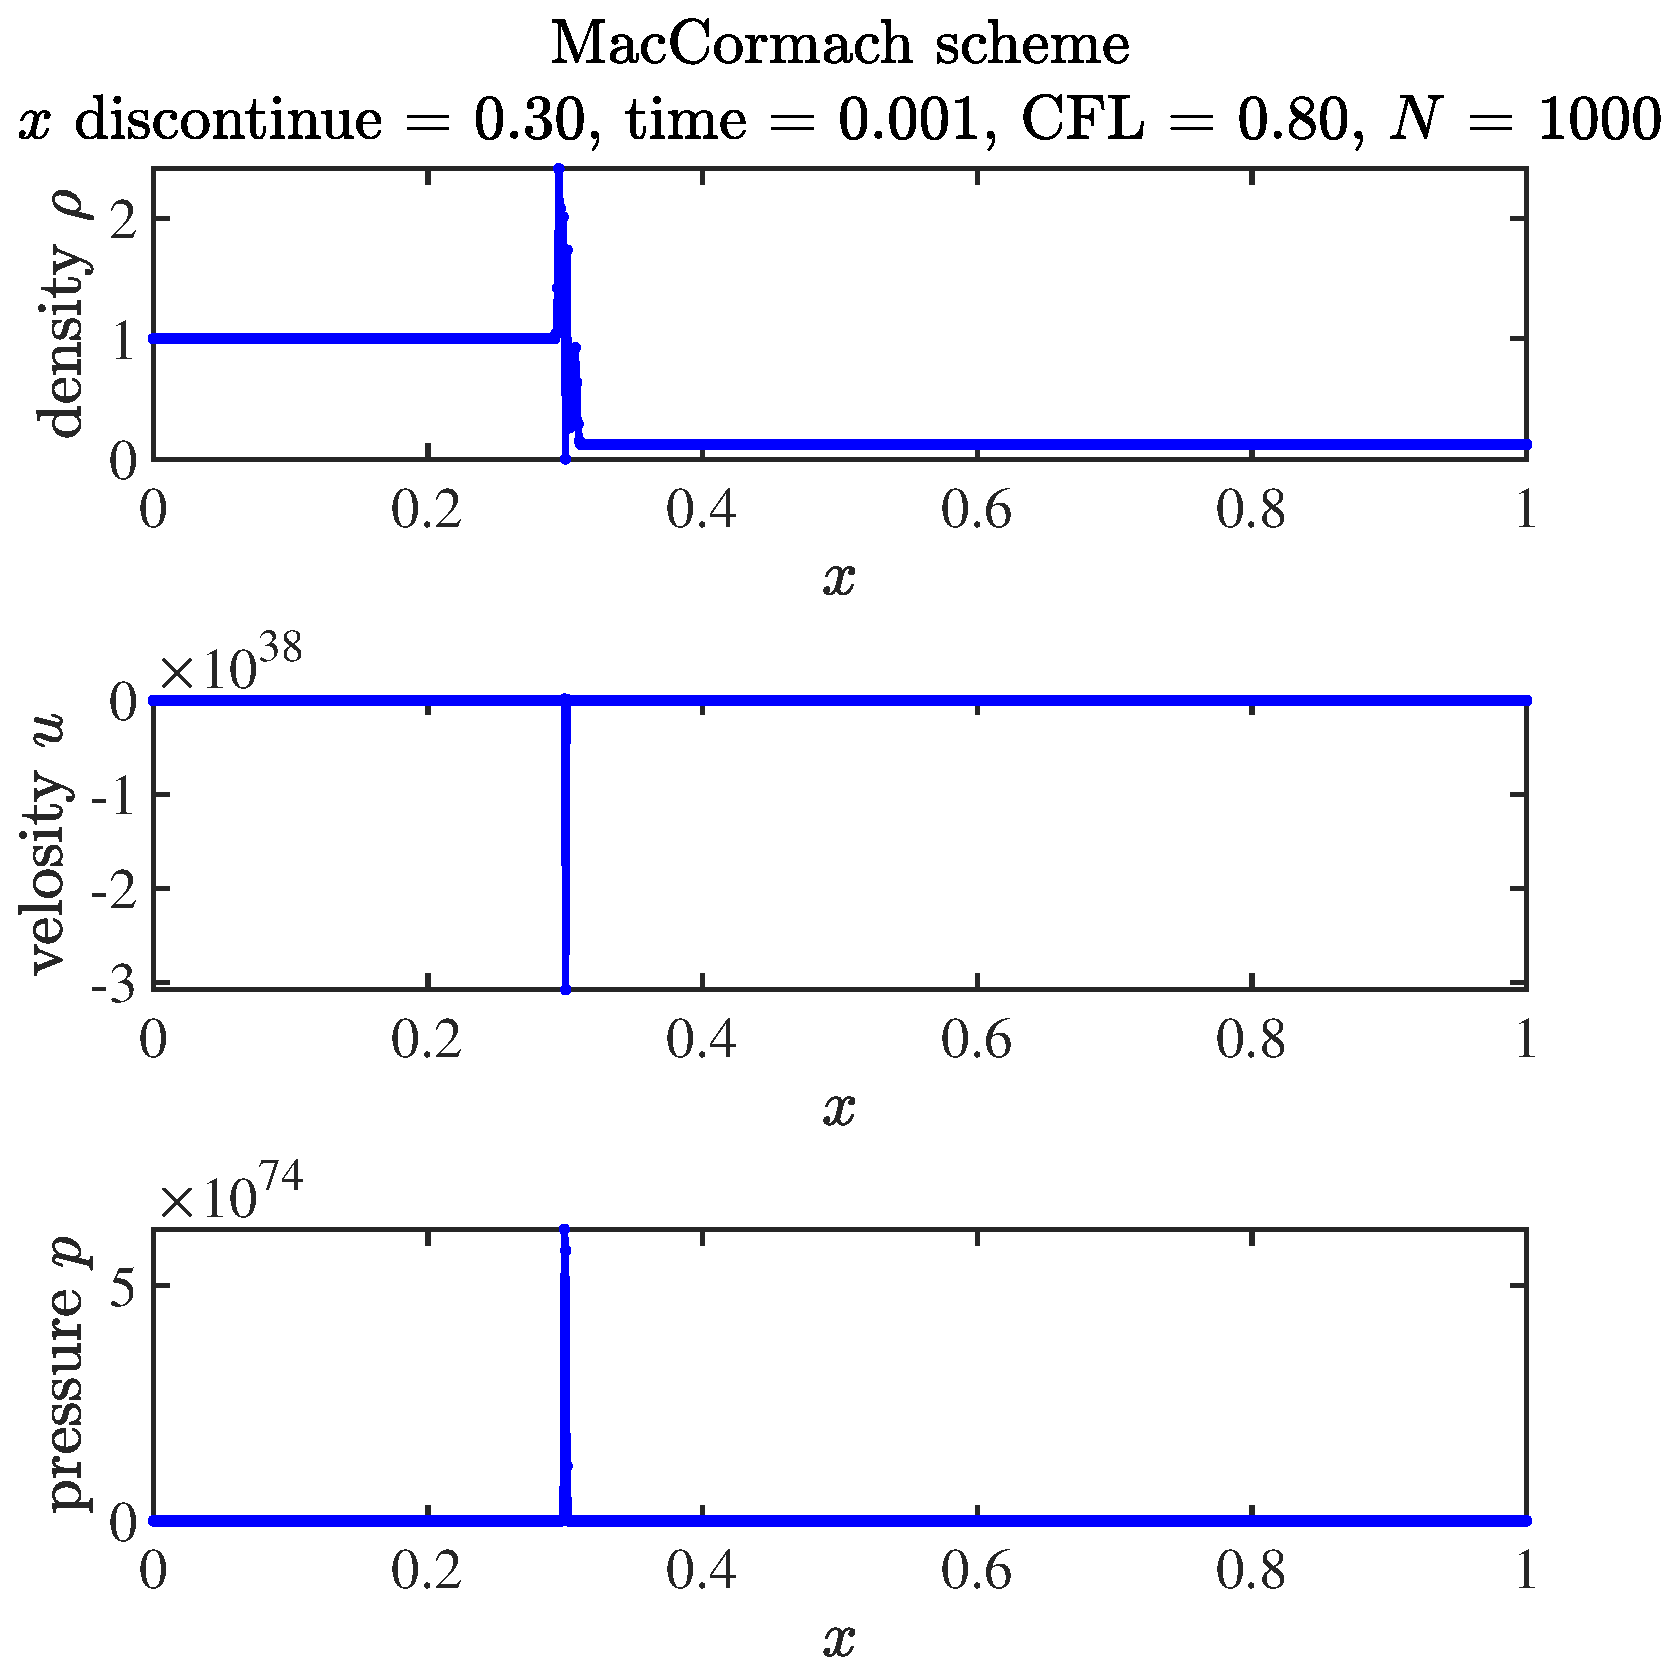
\includegraphics[width=9cm]{2Mac.eps}
	\vspace{20pt}
	\caption{Mac 格式计算结果。}
	\label{fig:2Mac}
\end{figure}

\subsection{Roe格式}

(P.L. Roe, JCP, 43, $1981,357-372 / 135,1997,250-258$ )
\begin{equation}
	\hat{\bm{F}}\left(\bm{U}_{j}, \bm{U}_{j+1}\right)=\frac{\bm{F}\left(\bm{U}_{j}\right)+\bm{F}\left(\bm{U}_{j+1}\right)}{2}-\frac{1}{2}\left|\hat{\bm{A}}_{j+1 / 2}\right|\left(\bm{U}_{j+1}-\bm{U}_{j}\right).
\end{equation}
其中 $|\hat{\bm{A}}|$ 定义为: $|\hat{\bm{A}}|=\bm{R}|\hat{\bm{\Lambda}}| \bm{R}^{-1}|,| \hat{\bm{\Lambda}} \mid=\operatorname{diag}\left\{\left|\hat{\lambda}_{1}\right|, \cdots,\left|\hat{\lambda}_{m}\right|\right\}, \bm{R}$为 $\hat{\bm{A}}$ 的右特征向量矩阵, $\hat{\Lambda}=\operatorname{diag}\left\{\hat{\lambda}_{1}, \cdots, \hat{\lambda}_{m}\right\}$, 即 $\bm{R}^{-1} \hat{\bm{A}} \bm{R}=\hat{\bm{\Lambda}}$,
\begin{equation}
	\begin{array}{c}
	\boldsymbol{R}=\left(\boldsymbol{R}^{(1)}, \boldsymbol{R}^{(2)}, \boldsymbol{R}^{(3)}\right)=\left(\begin{array}{ccc}
	1 & 1 & 1 \\
	u-a & u & u+a \\
	H-u a & \frac{1}{2} u^{2} & H+u a
	\end{array}\right).
	\end{array}
\end{equation}
\begin{equation}
	\bm{\Lambda} = \begin{pmatrix}
		u-a&&\\&u&\\&&u+a
	\end{pmatrix},
\end{equation}
\begin{equation}
	\hat{\bm{A}}_{j+1 / 2}\left(\bm{U}_{j+1}-\bm{U}_{j}\right)=\bm{F}\left(\bm{U}_{j+1}\right)-\bm{F}\left(\bm{U}_{j}\right).
\end{equation}
\begin{equation}
	\bm{U}^{n+1}_{j} =  \bm{U}^{n}_{j} - r \left( \hat{\bm{F}}^{n}_{j+\frac{1}{2}} - \hat{\bm{F}}^{n}_{j-\frac{1}{2}} \right).
\end{equation}
对于理性气体,通过如下方法构造$\hat{\bm{A}}$:
\begin{equation}
	\left\{
	\begin{aligned}
		\bar{\rho}&=\frac{\sqrt{\rho_{r}} \rho_{\ell}+\sqrt{\rho_{\ell}} \rho_{r}}{\sqrt{\rho_{\ell}}+\sqrt{\rho_{r}}}=\sqrt{\rho_{\ell} \rho_{r}}=\left[\frac{1}{2}\left(\sqrt{\rho_{r}} +\sqrt{\rho_{\ell}} \right)\right]^2, \\
		\bar{u}&=\frac{\sqrt{\rho_{\ell}} u_{\ell}+\sqrt{\rho_{r}} u_{r}}{\sqrt{\rho_{\ell}}+\sqrt{\rho_{r}}}, \\
		\bar{H}&=\frac{\sqrt{\rho_{\ell}} H_{\ell}+\sqrt{\rho_{r}} H_{r}}{\sqrt{\rho_{\ell}}+\sqrt{\rho_{r}}}.
	\end{aligned}\right.
\end{equation}
\begin{equation}
	\boldsymbol{A}(\boldsymbol{U})=\left(\begin{array}{ccc}
	0 & 1 & 0 \\
	\frac{\gamma-3}{2} u^{2} & (3-\gamma) u & \gamma-1 \\
	\frac{\gamma-2}{2} u^{3}-\frac{a^{2} u}{\gamma-1} & \frac{3-2 \gamma}{2} u^{2}+\frac{a^{2}}{\gamma-1} & \gamma u
	\end{array}\right),
\end{equation}
\begin{equation}
	a=\sqrt{\gamma p / \rho},\quad H=(E+p) / \rho,\quad p=(\gamma-1)\left(E-\frac{1}{2} \rho u^{2}\right).
\end{equation}
\begin{equation}
	\hat{\bm{A}}=\bm{A}(\bm{\bar{U}}).
\end{equation}
因为
\begin{equation}
	E=\frac{1}{\gamma}\left[H\rho+(\gamma-1)\frac{1}{2}\rho u^2\right],\quad p=H\rho - E,
\end{equation}
所以
\begin{equation}
	\bar{a}^2 = \frac{\gamma \bar{p}}{\bar{\rho}} = \gamma\frac{ \bar{H}\bar{\rho} - \bar{E}}{\bar{\rho}} = \gamma\frac{ \bar{H}\bar{\rho} - \frac{1}{\gamma}\left[\bar{H}\bar{\rho}+(\gamma-1)\frac{1}{2}\bar{\rho} \bar{u}^2\right]}{\bar{\rho}} =(\gamma-1) \left(\bar{H}-\frac{1}{2}\bar{u}^2\right).
\end{equation}


如\cref{fig:2Roe} 所示, Roe格式也无震荡。

\begin{figure}[htp]
	\centering
	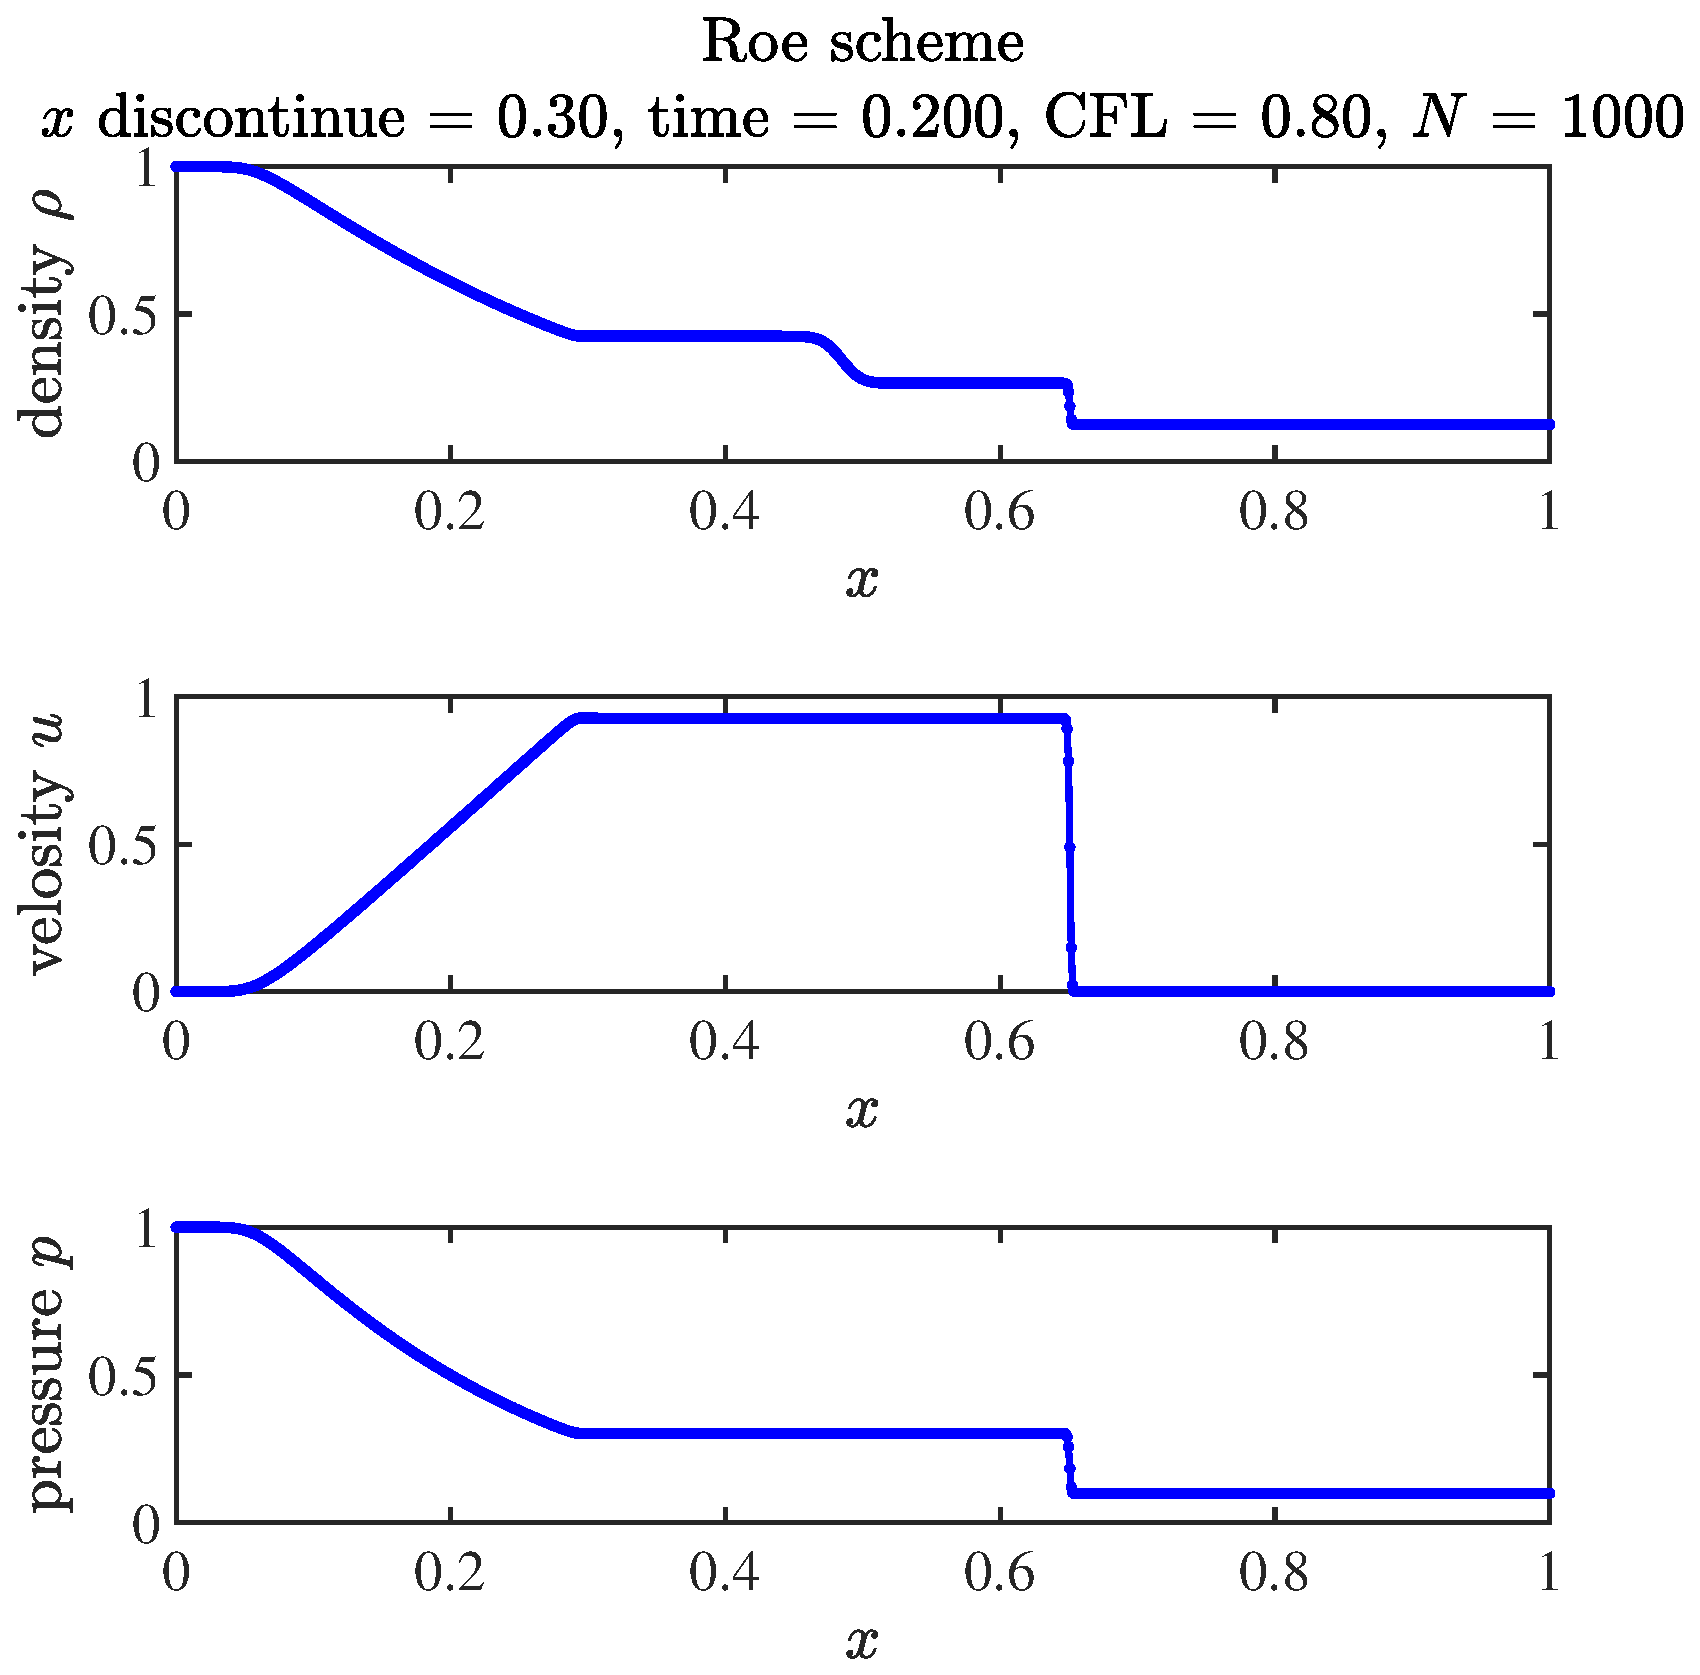
\includegraphics[width=9cm]{2Roe.eps}
	\vspace{20pt}
	\caption{Roe 格式计算结果。}
	\label{fig:2Roe}
\end{figure}


\section{2}

初 始 条 件
\begin{equation}
	(\rho, u, p)(x, 0)=\left\{\begin{array}{ll}
		(3.857143,2.629369,10.33333), & x<-4, \\
		(1+0.2 \sin (5 x), 0,1), & x \geq-4.
		\end{array}\right.
\end{equation}
计算区间为 $[-5,5]$, 其中在 $x=\pm 5$ 边界处 $\partial_{x} \rho=\partial_{x} u=\partial_{x} p=0 .$ 输出时刻 为 $t=1.8$.

如\cref{fig:4ini} 所示为初始条件.

\begin{figure}[htp]
	\centering
	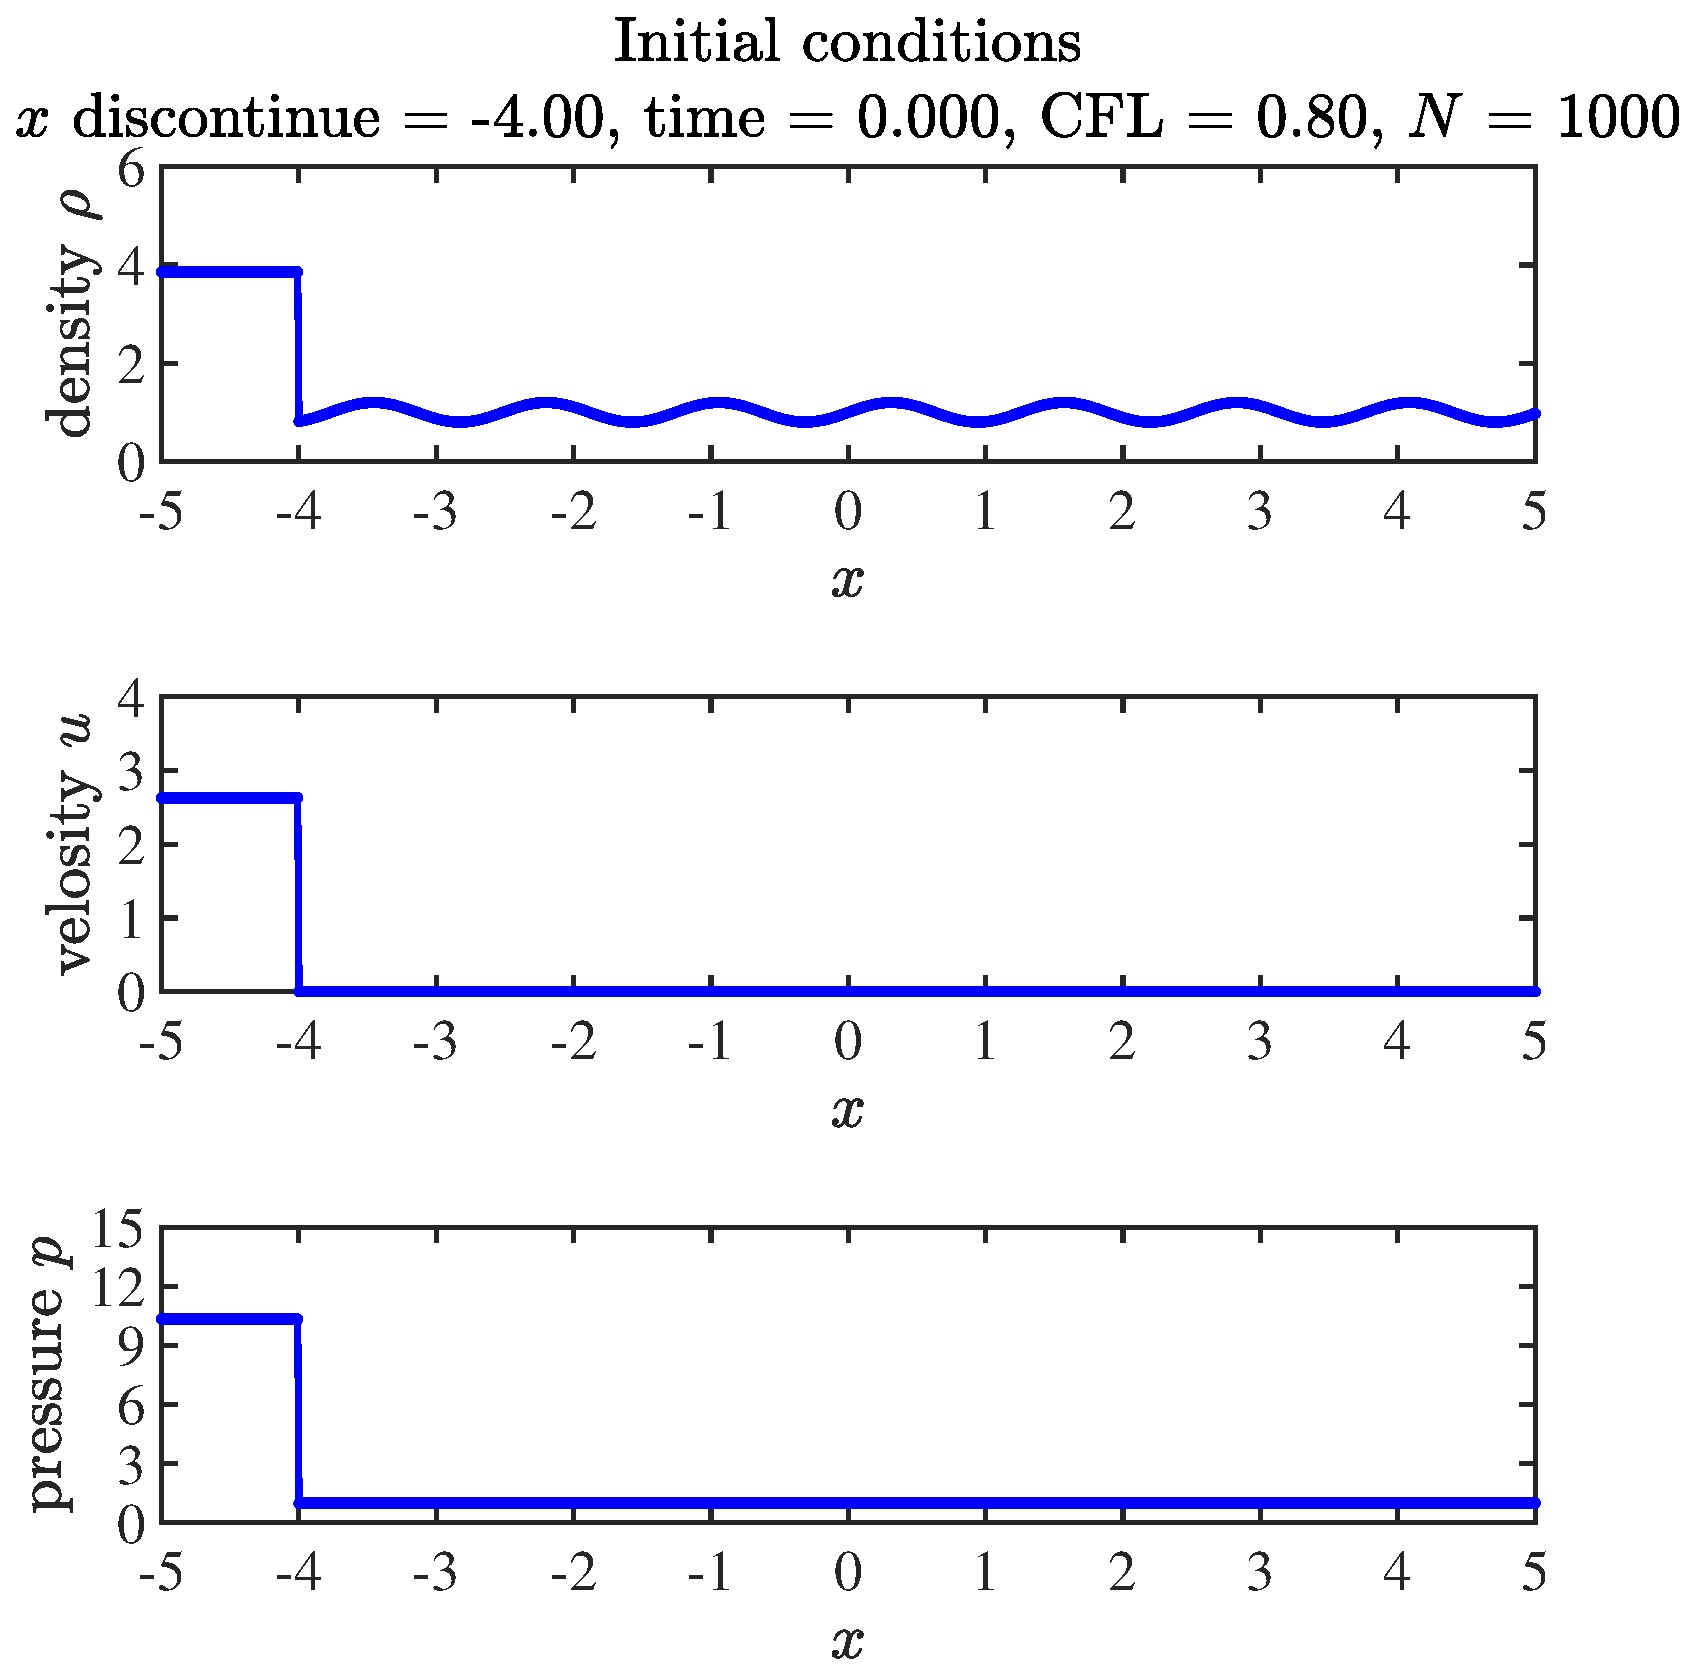
\includegraphics[width=9cm]{4Initial_conditions.eps}
	\vspace{20pt}
	\caption{初始条件。}
	\label{fig:4ini}
\end{figure}


\subsection{LF 格式}


如\cref{fig:4LF} 所示。可以发现,计算结果为一激波向右传播,耗散性较强,磨平了初始的密度浮动。
\begin{figure}[htp]
	\centering
	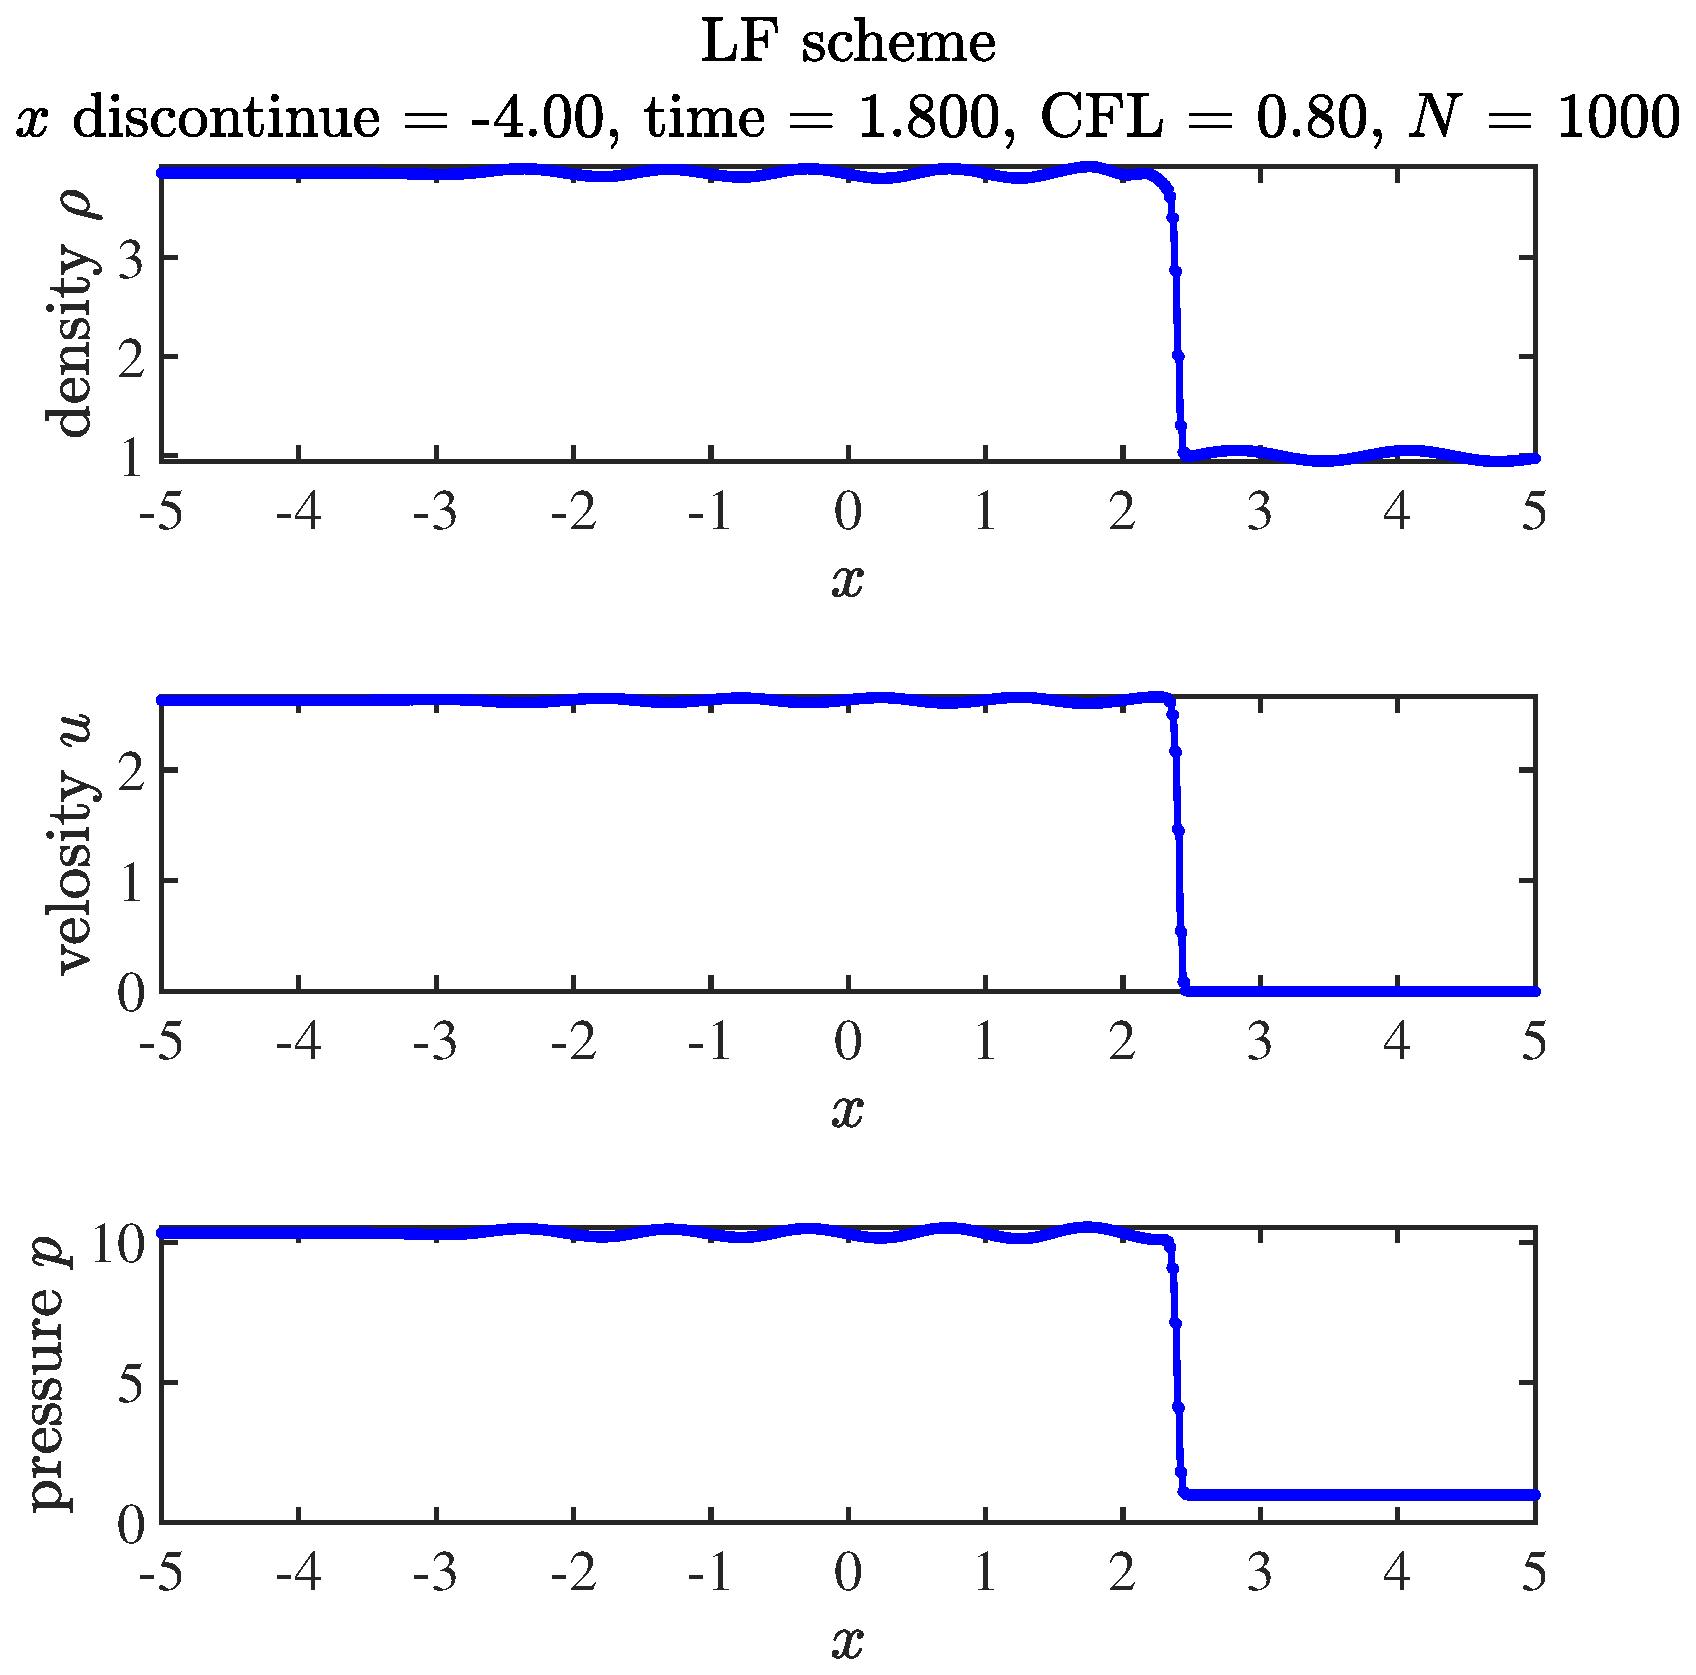
\includegraphics[width=9cm]{4LF.eps}
	\vspace{20pt}
	\caption{LF 格式计算结果。}
	\label{fig:4LF}
\end{figure}


\subsection{MacCormack格式}


如\cref{fig:4Mac} 所示, MacCormack格式稍微有一些震荡,尤其是在间断处间断明显,但是能完成计算。此格式的耗散性较弱。

\begin{figure}[htp]
	\centering
	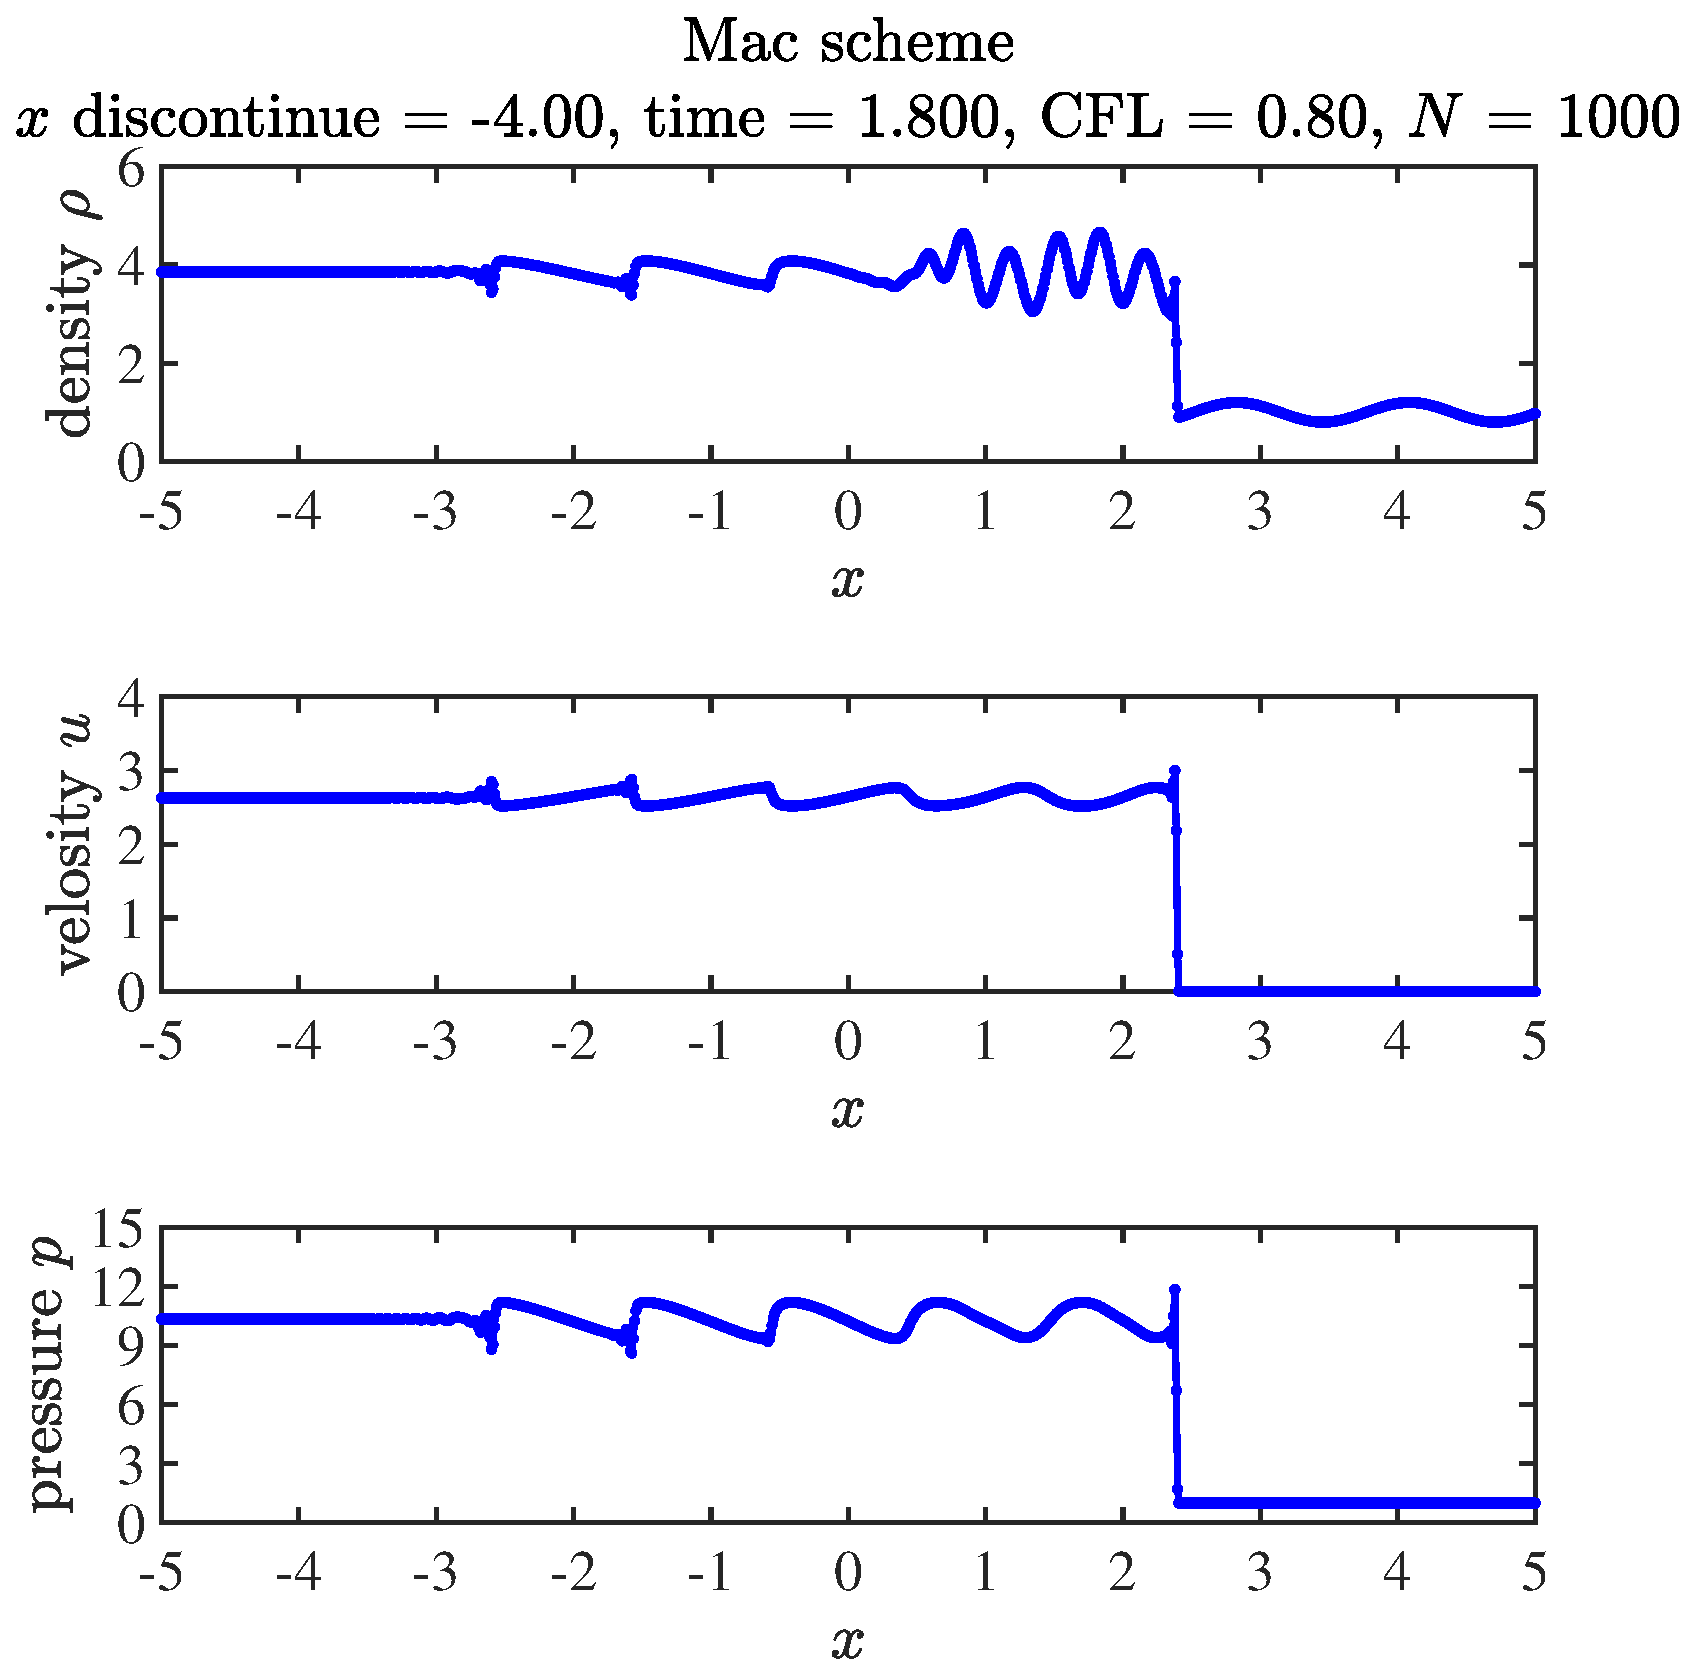
\includegraphics[width=9cm]{4Mac.eps}
	\vspace{20pt}
	\caption{Mac 格式计算结果。}
	\label{fig:4Mac}
\end{figure}

\subsection{Roe格式}

如\cref{fig:4Roe} 所示, Roe格式也无震荡。


\begin{figure}[htp]
	\centering
	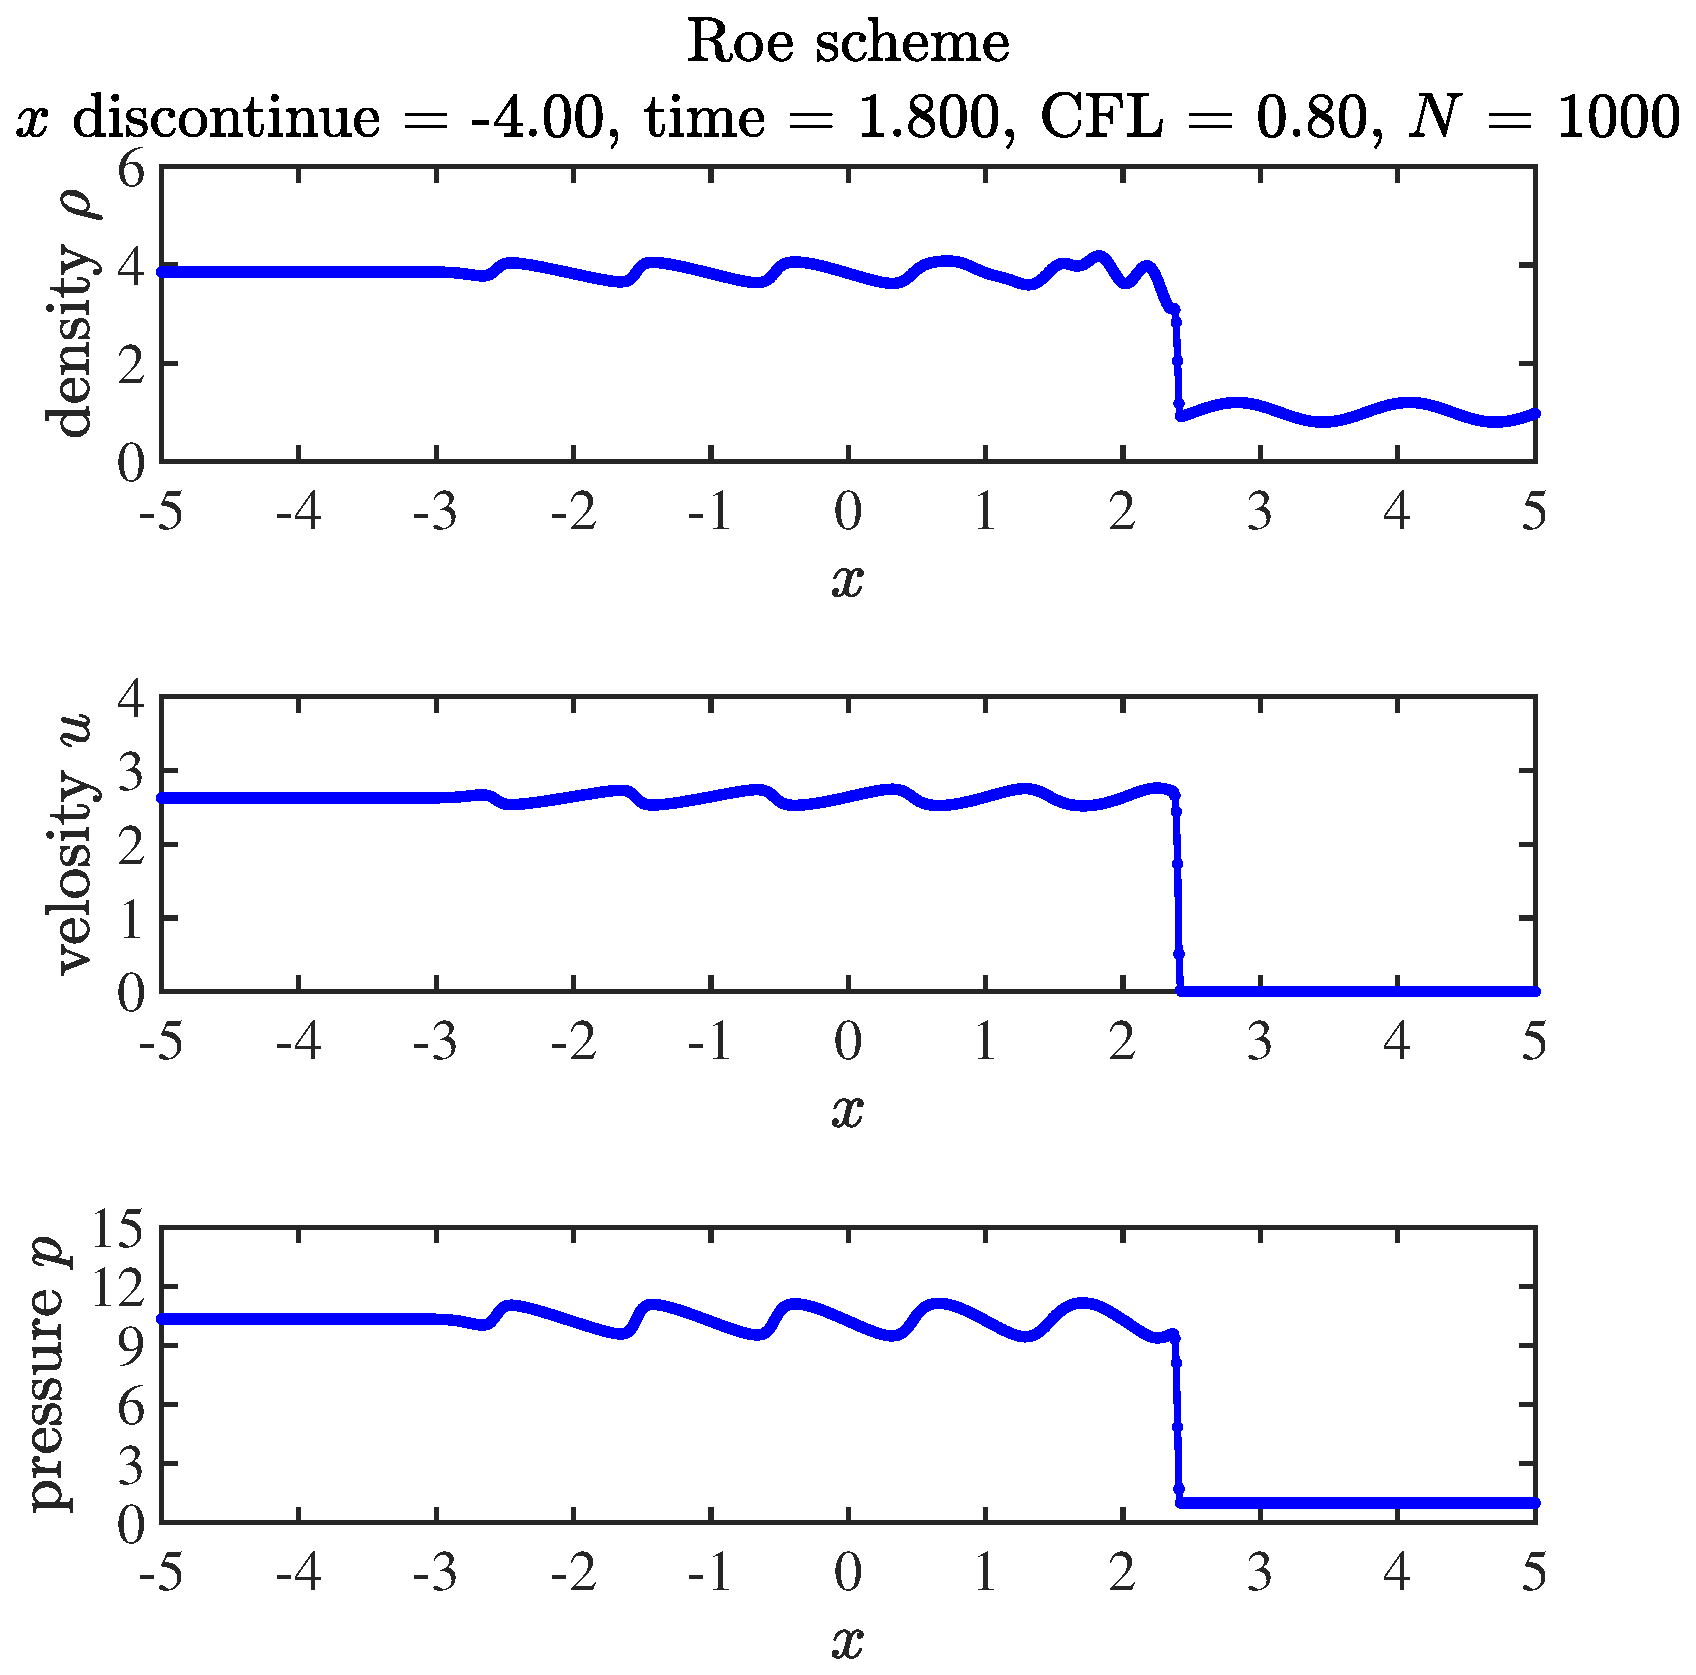
\includegraphics[width=9cm]{4Roe.eps}
	\vspace{20pt}
	\caption{Roe 格式计算结果。}
	\label{fig:4Roe}
\end{figure}













\bibliographystyle{plain}

\phantomsection

\addcontentsline{toc}{section}{参考文献} %向目录中添加条目,以章的名义
\bibliography{homework}

\end{document}
